% Chapter X

\chapter{Sviluppi Futuri} 
\label{ch:sviluppiFuturi}
Dall'analisi dei risultati delle stazioni è emerso che 
ci sono casi in cui l'interpolazione della retta sui $czf_{i,j,t}$ è imprecisa in quanto non ben allineati.
Altra limitazione del metodo è quella di non gestire più landslide nella stessa nearest zone.
Di seguito verrà illustrata una possibile soluzione a queste due problematiche. Avendo il modello digitale del terreno (DEM) da cui sono state ricavate le curve di livello del territorio abruzzese, si può fare un analisi approfondita del raster per ricavare più informazioni rispetto alle sole isoipse.   
Nel calcolo delle landslides anziché usare i centroidi $czf_{i,j,t}$ delle nearest zone si possono, attraverso l'analisi del DEM, ricavare i gradienti associati alle direzioni del terreno.
Le frecce in figura \ref{fig:gradienti}  rappresentano le direzioni di possibile frana del terreno. Per fare un collegamento con le definizioni del capitolo \ref{ch:notazioni}, ogni freccetta rappresenterebbe una landslide. \cite{gradienti}

\begin{figure}[H]
	\centering
	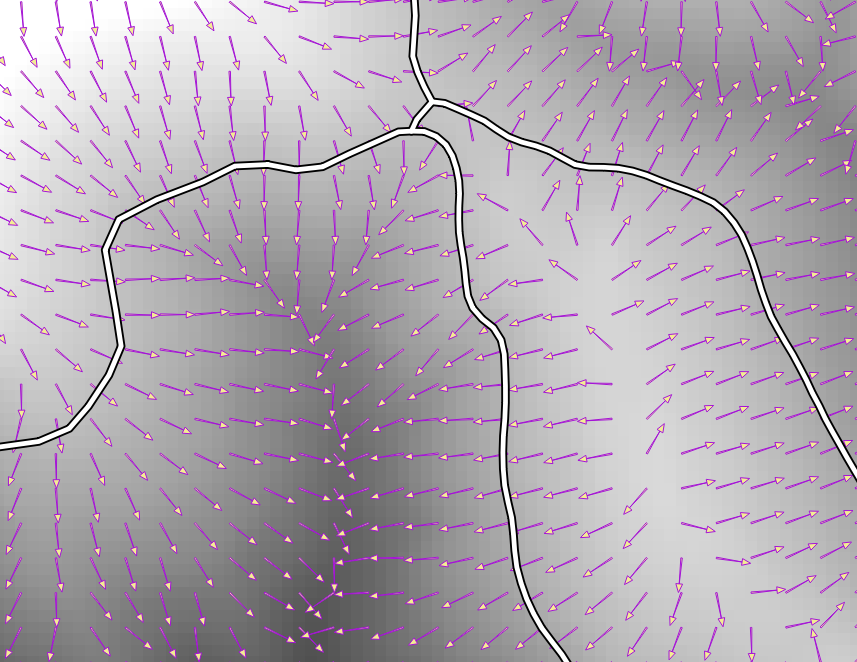
\includegraphics[width=0.7\textwidth]{images/gradienti.png}
	\caption{Gradienti ricavati a partire da file raster (DEM)}
	\label{fig:gradienti}
\end{figure}
Per poter gestire più landslide all'interno di una zone essa potrebbe essere partizionata in tante zones più piccole in modo tale che ognuna di esse contenga solo una direzione di caduta.
Ognuna delle zones ha associato il gradiente che indica la sua direzione di caduta.
Ciò permetterebbe di creare delle landslide molto più coerenti con l'andamento dei pendii del terreno.
 


